\documentclass[12pt,a4paper]{report}

\usepackage{geometry}
\usepackage{graphicx}
\usepackage{longtable}
%\usepackage{pgfgantt}
\usepackage[dutch]{babel}
\usepackage{url}
%\usepackage{pgf,pgfplots}
%\usetikzlibrary{fit,calc}
%\usepgfplotslibrary{external}

\geometry{a4paper}

\newcommand{\boxplot}[6]{%
	%#1: center, #2: median, #3: 1/4 quartile, #4: 3/4 quartile, #5: min, #6: max
	\filldraw[fill=white,line width=0.2mm] let \n{boxxl}={#1-0.1}, \n{boxxr}={#1+0.1} in (axis cs:\n{boxxl},#3) rectangle (axis cs:\n{boxxr},#4);   % draw the box
	\draw[line width=0.2mm, color=red] let \n{boxxl}={#1-0.1}, \n{boxxr}={#1+0.1} in (axis cs:\n{boxxl},#2) -- (axis cs:\n{boxxr},#2);             	% median
	\draw[line width=0.2mm] (axis cs:#1,#4) -- (axis cs:#1,#6);                                                                           							% bar up
	\draw[line width=0.2mm] let \n{whiskerl}={#1-0.025}, \n{whiskerr}={#1+0.025} in (axis cs:\n{whiskerl},#6) -- (axis cs:\n{whiskerr},#6);        % upper quartile
	\draw[line width=0.2mm] (axis cs:#1,#3) -- (axis cs:#1,#5);                                                                           							% bar down
	\draw[line width=0.2mm] let \n{whiskerl}={#1-0.025}, \n{whiskerr}={#1+0.025} in (axis cs:\n{whiskerl},#5) -- (axis cs:\n{whiskerr},#5);        % lower quartile
}


\begin{document}

%  Titelblad

\begin{titlepage}

\fontsize{12pt}{14pt}\selectfont

\begin{center}

\vspace{1cm}

\fontsize{14pt}{17pt}\selectfont
% De Faculteit:
\textsc{P\&O Computerwetenschappen - Verslag \\Team Platinum}
\fontsize{12pt}{14pt}\selectfont
\vspace{0.3cm}

\vspace{1.2cm}

%Het academiejaar: aanpassen!
Academiejaar 2011--2012

\vspace{2.8cm}

\fontsize{17.28pt}{21pt}\selectfont

% De titel van de thesis:
{\textsc{Pac-Man in de echte wereld,\\ met behulp van Lego Mindstorms}}

\fontseries{m}
\fontsize{12pt}{14pt}\selectfont

\vspace{2cm}


\includegraphics[height=10cm]{resources/Logo-Kul}

\end{center}
\end{titlepage}

\thispagestyle{empty}

\tableofcontents

\begin{abstract}
Tijdens de uitwerking van dit jaar-overschrijdend groepswerk, bouwen wij een autonome robot met behulp van Lego Mindstorms. Voor de programmatie wordt beroep gedaan op Lejos, een Open Bron project dat een minimale JAVA virtuele machine heeft gemaakt die de plaats kan innemen van de standaard programmatie omgeving van Lego.

Naast de doelstelling om kennis te maken met het ontwikkelen van een autonome robot, willen we in dit project ook ervaring opdoen i.v.m. het werken in teamverband aan een middelgroot softwareproject. Hierbij zijn organisatie van werk, planning, analyse, architectuur,... belangrijke begrippen.

In het tweede semester wordt hier nog eens de nood aan samenwerking toegevoegd. Het traject van de autonome robot blijft behouden, maar de verschillende robots zullen nu moeten samen werking om een gemeenschappelijk doel te bereiken. Om deze samenwerking in goede banen te leiden werd een scheidsrechtercommissie in het leven geroepen om de beslissingen te nemen die voor alle teams van belang zijn. Het doel van dit semester ligt in het insluiten van een ``Pac-Man''-robot bestuurd door het didactisch team, dit met behulp van vier autonome ``ghosts''.

In het eerste semester werkten we reeds in een parallel traject aan een simulatieomgeving. Aan de hand van deze omgeving waren we in staat om met meerdere teamleden in parallel een robot te ontwikkelen zonder nood aan een fysieke. Nu is het ontwikkelen van deze simulator deel geworden van de verdere opdracht en dienen we dus de nodige aanpassingen te doen om het Pac-Man-spel in de computer te simuleren. Het gebruik van een simulator is evident, aangezien we niet kunnen verwachten alle fysieke testen uit te voeren met de 4 teams tegelijk.
\end{abstract}

\chapter{Inleiding}

Het project wordt zoals in het eerste semester begeleid door het gebruik van tussentijdse demo's. Het finale doel is om zo optimaal mogelijk samen te werken met vier teams om de Pac-Man in te sluiten, hoewel we ten alle tijden autonoom beslissingen nemen.

Het doel van de eerste demo is een versimpelde vorm van het einddoel waarbij we een stilstaande Pac-Man zoeken binnen het doolhof. De simulator dient ook reeds beschikbaar te zijn. Voor de tweede demo mag de commissie beslissen welke doelstellingen passen in het verdere proces richting het einddoel.

Duidelijk is dat we er in geslaagd zijn om zeer herbruikbare code te produceren in het eerste semester. Iedereen is ondertussen vertrouwd geraakt met de volledige architectuur. Aangezien we duidelijk te maken hebben met een grote diversiteit aan kleine taken, gebeurt het grootste deel van de taakverdeling week op week.

Het verslag is duidelijk verschillend opgebouwd ten opzichte van het vorige semester en kiest voor een onderverdeling in subsecties per demo binnen een context van hoofdstukken. De opbouw van deze hoofdstukken is duidelijk erg gelijkend hoewel natuurlijk de inhoud veranderd is t.o.v. het eerste semester. Nieuw zijn natuurlijk de stukken over de strategie ivm de opgegeven spelomgeving, over de samenwerking en over de finale analyse van het jaarproject.

\chapter{Probleemstelling}

De doelstellingen van de demo's worden hier achtereenvolgens beschreven, zij liggen in de lijn van het ontwerpproces richting een autonome ghost, die samen met de drie anderen probeert de Pac-Man in te sluiten.

\section{Demo 1}

Het probleem dat we eerst aanpakken is het zo efficient mogelijk in kaart brengen van een onbekende omgeving met behulp van de vier ghosts, belangrijk hierbij is dat de in beeld gebrachte wereld overeenkomt met de realiteit. Tijdens de demo gebruiken we een hybride simulator, onze eigen robot bestaat in de fysieke wereld, de andere drie zijn virtueel en worden vertegenwoordigd door drie virtuele ``ghost'' die in simulator ``leven''.

De ``ghosts'' hebben geen enkele informatie over het doolhof waarin ze zich bevinden, noch over hun positie, noch over hun ori\"entatie. Verder staat de Pac-Man stil in het parcours en dient hij enkel gevonden te worden. We dienen ook aan te tonen dat het door de commissie afgesproken communicatieprotocol ge\"implementeerd is.

Elk team wordt tijdens de demo afzonderlijk beoordeeld.
 
\section{Demo 2}
 
Dit dient nog afgesproken te worden door de commissie.

\section{Demo 3}

\subsection{Verkenning}

De robots rijden in een onbekend doolhof. Alle info die verzameld wordt door de vier ghosts draagt bij tot het cre\"eren van een individuele map die mogelijk inconsistenties bevat. Alle juiste info over het doolhof zal direct bijdragen tot het hoofddoel, namelijk het vangen van de pac-man. Elke robot communiceert zijn gevonden informatie en probeert zo veel mogelijk informatie te verzamelen over de rond hem onbekende wereld, het falen van \'e\'en van de robots kan reeds fataal zijn voor het snel kunnen opbouwen van een verkende omgeving. We proberen dus een zo robuust mogelijke robot te maken die zo effici\"ent mogelijk zijn eigen info verzamelt en met de nodige voorzichtigheid andere informatie hierin verwerkt.

\subsection{Pac-Man}

Het Pac-Man spel zelf kunnen we winnen door alle vluchtwegen van de Pac-Man af te sluiten. Dit houdt in dat alle omliggende sectoren door een ghost bezet wordt of afgeschermd worden door een muur. Men wint enkel als alle robots die meewerken aan de insluiting ook effectief aangeven dat ze gewonnen hebben. De probleemstelling vereist dus een effectieve samenwerking, waarbij een consensus moet bereikt worden over de verzamelde informatie en de te volgen strategie.

\chapter{Scheidsrechtercommissie}

Deze commissie staat in voor het nemen van beslissingen die betrekking hebben op afspraken tussen de verschillende teams en het didactische team. Hierbij kunnen we deze beslissingen groeperen in:
\begin{itemize}
	\item De verdere regels waarmee de spelomgeving beperkt wordt.
	\item Afspraken die noodzakelijk zijn voor de samenwerking van de teams.
\end{itemize}

\section{Spelregels}

\subsection{Spelwereld}

De spelwereld bestaat uit aangepaste panelen uit het eerste semester. Er is een raster van witte lijnen ge\"introduceerd waar mogelijks muren kunnen staan. Dit komt neer op een mogelijke herschaling van de panelen met een factor vier. Deze nieuwe minimumeenheid aan oppervlakte noemen we sectoren. Deze zijn belangrijk voor de plaatsbepaling binnen het doolhof. De doolhof is volledig ommuurd en de absolute afmetingen worden op voorhand gegeven.

\subsection{Pac-Man}

De Pac-Man wordt zichtbaar gemaakt door een infrarood-beacon dat kan opgemerkt worden met behulp van de voorziene IR-sensor. Het didactisch team kiest waar deze vertrekt en bestuurt hem tijdens de demo's. Hij mag enkel bewegen op sectoren waar zich geen ``ghosts'' beevinden.

De beweging van Pac-Man is beperkt tot het rechtdoor oversteken van de witte lijnen die de sectoren scheiden.

\subsection{Ghosts}

De ghosts vertrekken op de vier hoekpunten van de doolhof, zodat de verkenning van het doolhof zo snel mogelijk van start kan gaan. De ori\"entatie van de robot is onbekend hoewel de hoek t.o.v. het assenstel wel een veelvoud is van 90 graden.


\section{Communicatieprotocol}

We verwijzen naar de offici\"ele documentatie van het Ghost Protocol. Ten tijde van het schrijven van dit verslag was versie 1.0 beschikbaar. Het Ghost Protocol is het resultaat van een werkgroep door de commissie aangesteld. In dit deel van het verslag belichten we de positieve en de negatieve punten van het voorgestelde protocol en bespreken de voor- en nadelen voor onze eigen ontwikkeling.

\subsection{Voordelen}

TODO: Michiel: Als jij er in slaagt om iets positiefs te zeggen ;-)

\subsection{Nadelen}

In het algemeen ondervinden we geen nadelen van de beslissingen die genomen zijn. Aangezien wij voldoende informatie kunnen verzamelen met een kleine subset, zal het volledige protocol slechts een marginale implementatiekost met zich meebrengen.

TODO: Michiel: Zoals eerder vandaag besproken de puntjes omtrent overbodigheid en onvolledigheid.

\chapter{Robot}

\section{Demo 1}

\subsection{Fysiek ontwerp}

Door de veranderde specificaties van het doolhof en de extra infrarood sensor, moesten enkele wijzigingen gemaakt worden aan de fysieke robot. Zo zijn de druksensoren verwijderd om een sensorpoort vrij te maken voor de infrarood sensor. Bovendien is het in dit project noodzakelijk om precies mogelijk door het midden van de sectoren te rijden, en touch-sensoren passen niet in deze strategie. Aangezien het doolhof minder breed is (sectoren zijn 40 centimeter in plaats van 80) zijn de extra wielen weggehaald om het geheel iets slanker te maken wat een eenvoudigere navigatie mogelijk maakt.

Verder is ook de motor, die de sonar laat draaien, iets naar onder verplaatst en naar het midden. Hierdoor hebben we uit de verbinding tussen de motor en de sensor de tandwielen kunnen verwijderen waardoor de sensor rechtstreeks op de motor zit. Om eenvoudiger de ouput van de robot te kunnen lezen, is de brick omgedraaid, zodat het display zich nu aan de onderzijde van de robot bevindt.

\subsection{IR-sensor}
De Infrarood sensor werd vooraan in het midden van de robot aangebracht. Net boven de lichtsensor. Het uitlezen van deze sensor zorgde voor een aantal problemen. De maximale gemeten afstand kwam niet overeen met de specificatie van de IR-bal en sensor. Het bleek dat de Lejos implementatie verouderd was en niet alle mogelijkheden van de sensor ondersteunde. Met behulp van de broncode van Lejos versie 9.0 en enkele aanpassingen, is ons team er in geslaagd de verschillende sensormodi te activeren.

Uit testen bleek dat er voor de bol verschillende AC modi en \'e\'en DC modus is. De sensor heeft \'e\'en AC modus en \'e\'en DC modus. Er bleek dat de AC modus van de bol die speciaal voor de sensor ontwikkeld was het beste werkte. De sensor had dan een reikwijdte van 5 meter in tegenstelling tot ongeveer 80 cm bij andere modi.

\begin{figure}
\begin{center}
 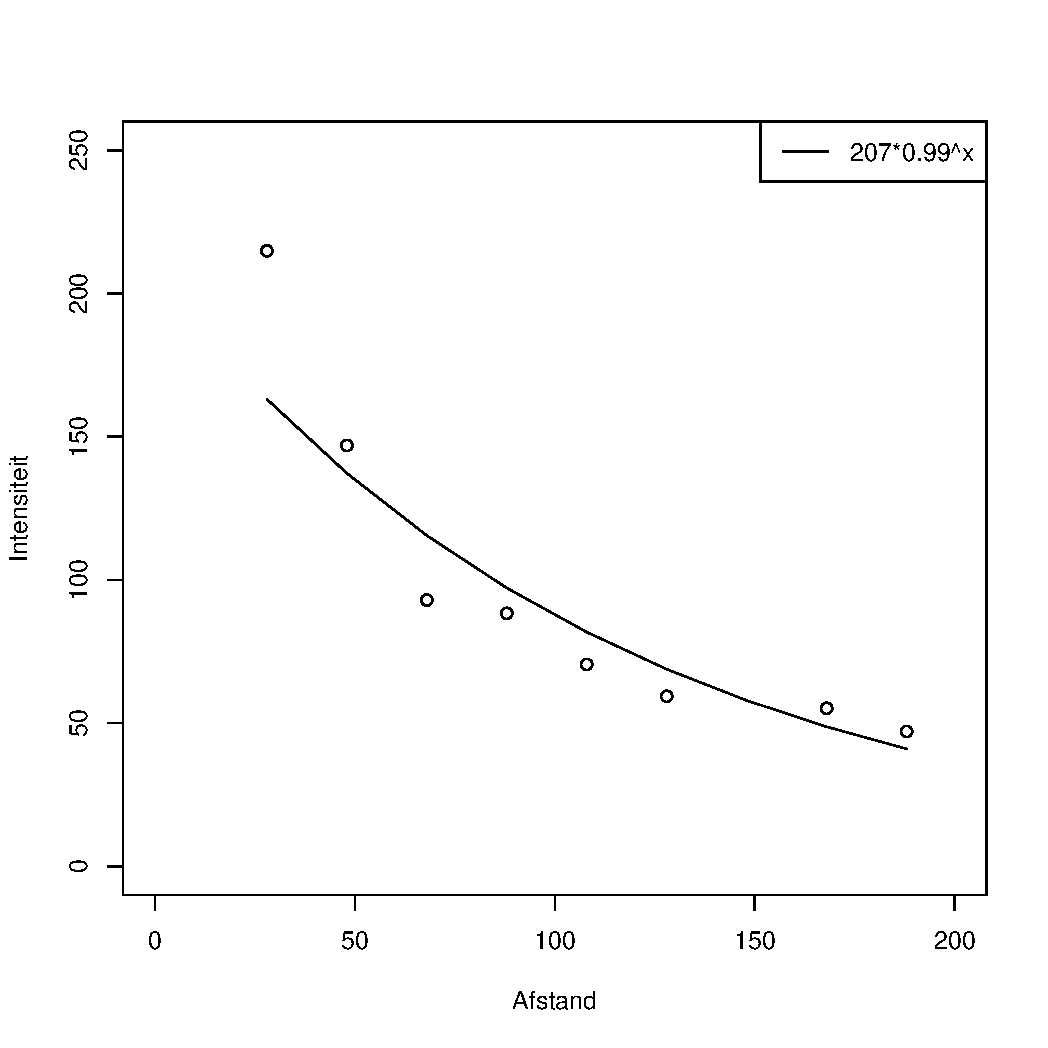
\includegraphics[width=\textwidth]{./resources/plotIR.pdf}
 \caption{De meetwaarden van de IR-sensor volgens een bepaalde afstand \label{fig:plotIR}}
 % plotIR.pdf: 504x504 pixel, 72dpi, 17.78x17.78 cm, bb=0 0 504 504
\end{center}
\end{figure}


 De sterkte is bij weerkaatsing herkenbaar lager dan bij een rechtstreekse detectie (zie grafiek). Men kan dus eventueel ook aan de hand van de signaalsterkte herkennen of de pacman zich achter een hoek bevindt. In dit geval kan deze meting best genegeerd worden. Het reconstrueren van een weerkaatsingpatroon een zeer moeilijke opgave.

In grafiek \ref{fig:plotIR} kan men zien dat de gemeten lichtsterkte exponentieel afneemt ten opzichten van de afstand tot de lichtbron.
Hieruit zou men kunnen een schatting bepalen van de afstand tot de bron. In grafiek \ref{fig:boxplotIR} kan men de variatie van de IR-sensor zien voor verschillende afstanden. We zien dat de varianties zeer klein zijn in vergelijking met de lichtsterkte. Een afstandsschatting lijkt dus goed mogelijk.

Uit testen blijkt dat een significante hoeveelheid van het IR licht via weerkaatsingen door de infraroodsensor gedetecteerd wordt.
De sterkte is bij weerkaatsing herkenbaar lager dan bij een rechtstreekse detectie (zie grafiek \ref{fig:boxplotSpiegeling}).  Men kan dus eventueel ook aan de hand van de signaalsterkte herkennen of de pacman zich achter een hoek bevindt. In dit geval kan deze meting best genegeerd worden. Het reconstrueren van een weerkaatsingpatroon een zeer moeilijke opgave.

\begin{figure}
\begin{center}
 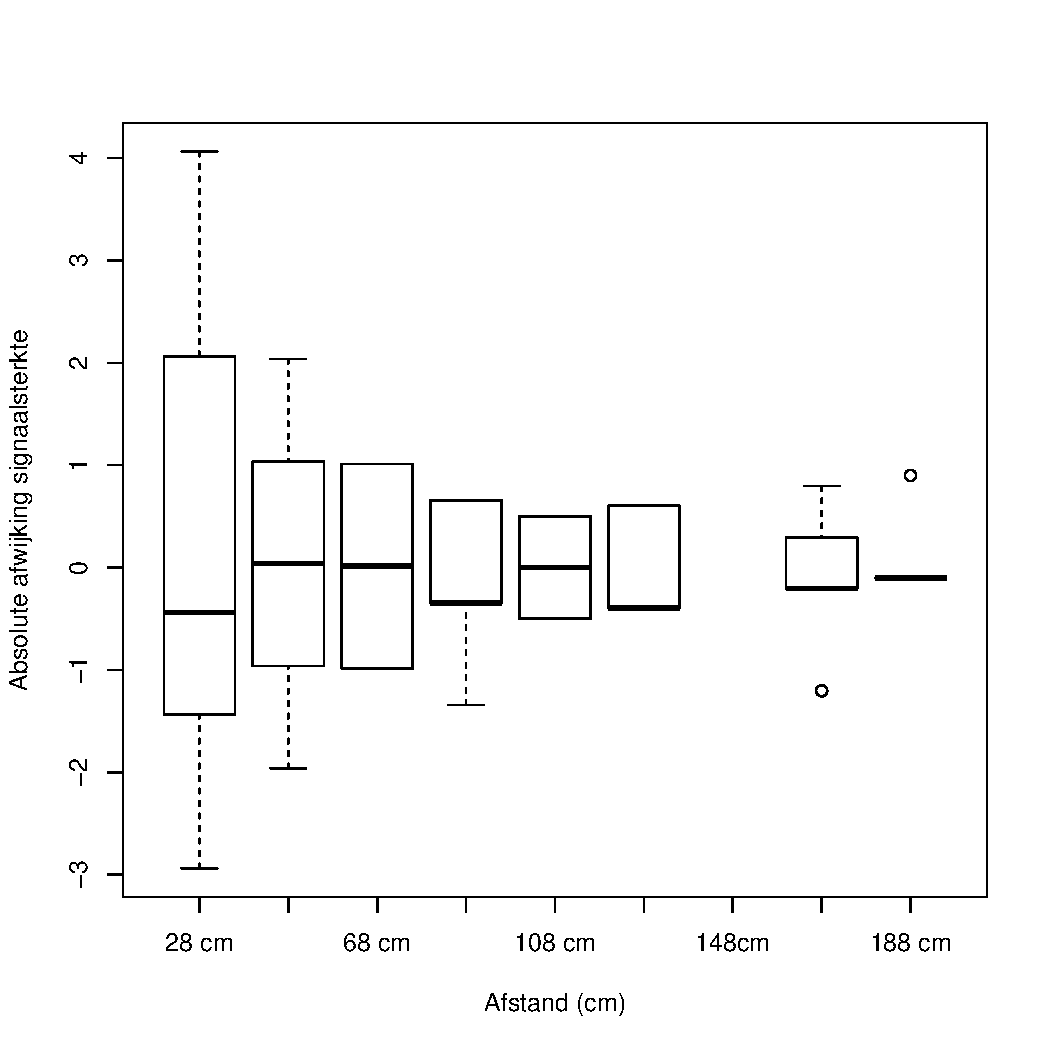
\includegraphics{./resources/bloxplotIR.pdf}
 \caption{Sensorwaarden van de IR-sensor bij verschillende afstanden \label{fig:boxplotIR}}
\end{center}
\end{figure}

\begin{figure}
\begin{center}

 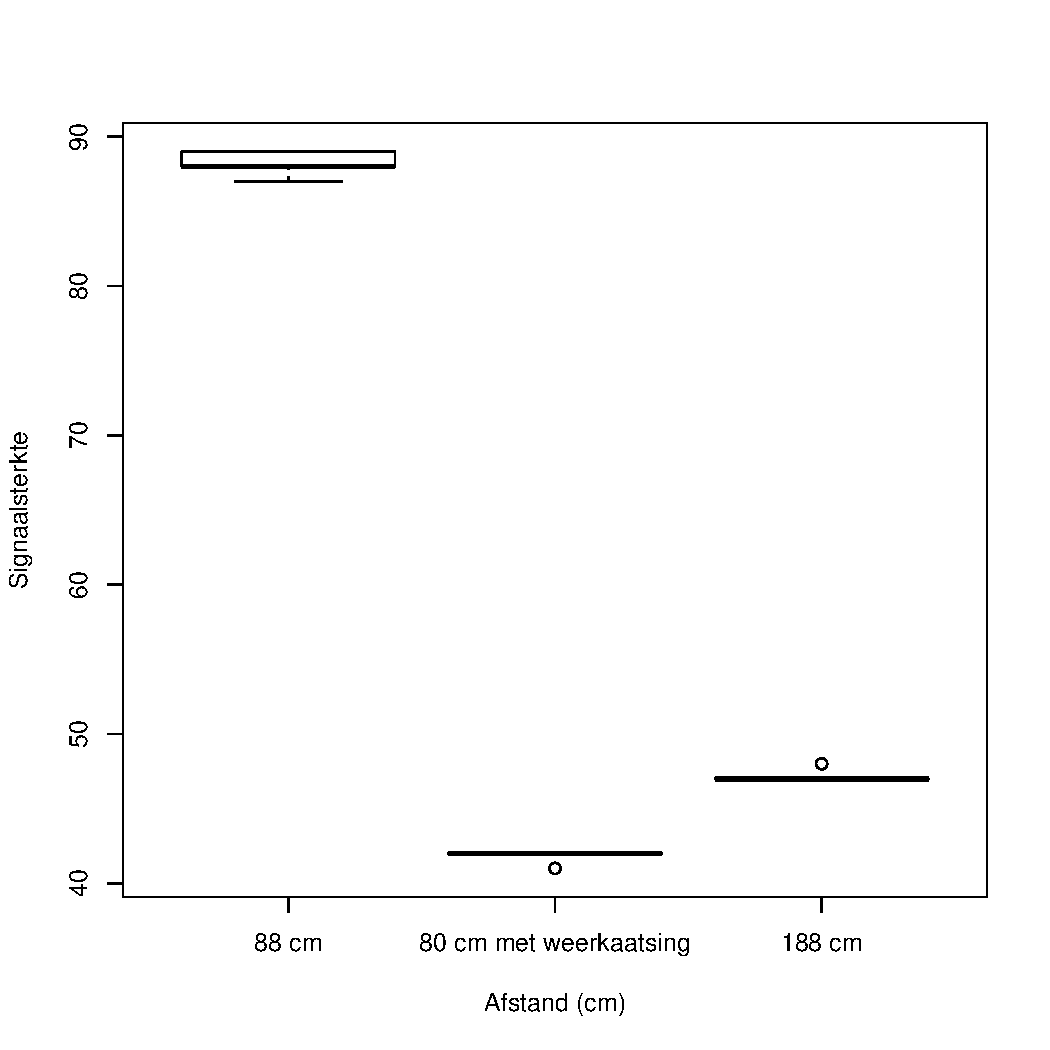
\includegraphics{./resources/boxplotSpiegeling.pdf}
 \caption{Sensorwaarden van de IR-sensor bij weerkaatsing en verschillende afstanden 
\label{fig:boxplotSpiegeling}}

\end{center}
\end{figure}

Een nadeel van zo'n filtering is dat deze de afstand waarop geschat kan worden inperkt. Zoals men kan zien op de grafiek \ref{fig:boxplotSpiegeling}, kunnen we geen afstanden van meer dan 160 cm (4 sectoren) onderscheiden van weerkaatsingen. Voor demo 2 en 3 zal moeten afgewogen worden wat de beste oplossing is: een grotere gemeten afstand maar misschien niet nauwkeurig, of een grotere zekerheid garanderen. Hier zal ook rekening gehouden moeten worden met de andere teams. 

\section{Demo 2}

Dit deel wordt later toegevoegd.

\section{Demo 3}

Dit deel wordt later toegevoegd.

\chapter{Strategie}

Aangezien wij ons slechts sinds enkele maanden begeven op het terrein van autonome robots en artifici\"ele intelligentie, zou het dom zijn te veronderstellen dat er ons nog niemand is voor gegaan. We hebben daarom een literatuurstudie rond de concepten van Pac-Man en autonome ``ghosts'' gedaan.

We vonden een paper omtrent ``Collaborate Diffusion''\footnote{\url{http://www.cs.colorado.edu/~ralex/papers/PDF/OOPSLA06antiobjects.pdf}}. Hierin wordt voorgesteld om een vorm van ``Hill Climbing'' \footnote{\url{http://en.wikipedia.org/wiki/Hill_climbing/}} toe te passen om zo verschillende autonome ``ghosts'' toe te laten samen te werken om een ``Pac-Man'' te achtervolgen. Hierbij hebben zij geen nood aan bijkomende onderlinge communicatie naast de informatie over de wereld.

Ondanks het feit dat we geen overeenstemming met de andere teams konden bereiken om allen dit algoritme te implementeren, blijft het een zeer interessant algoritme om toe te passen voor het bepalen van ons eigen pad.

\section{Achtervolgstrategie}

Wanneer de Pac-Man gezien wordt stuurt deze een ``geur'' uit. Deze plant zich langs gekende sectoren voort. Dit wordt gedaan door het gemiddelde van de 4 omliggende sectoren te berekenen, indien er een muur staat is de waarde 0. Zo ontstaat er een hoogte-kaart met aan de top een Pac-Man. De Ghosts kunnen nu aan de hand van een eenvoudig ``Hill Climbing'' algoritme een optimale weg volgen naar de Pac-Man.

Wanneer een ``ghost'' de Pac-Man opmerkt, kan deze positie op de kaart een zeer hoge waarde gegeven worden. Deze kaart wordt vaak herberekend en de geur van een Pac-Man zal dus snel verdwijnen. En dit is zoals het in de realiteit ook zal zijn. De Pac-Man beweegt zich doorheen het doolhof en zal niet op \'e\'en plek blijven wachten. Als een Pac-Man meerdere keren gezien wordt zal zijn positie ook een constantere ``geur'' verspreiden, waardoor de ``ghosts'' van alle kanten op hem kunnen naderen. Figuur \ref{fig:hillclimbing1} toont het principe aan de hand van een visualisatie van de hoogte of geur van de Pac-Man door middel van een kleurenpallet. Hierbij zijn hoge waarden rood gekleurd en lage waarden violet.

\begin{figure}[htbp]
  \centering
  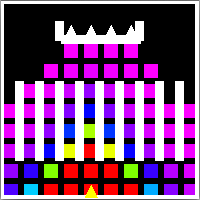
\includegraphics[width=50mm]{resources/hillclimbing1.png}
  \caption{Hill Climbing}
  \label{fig:hillclimbing1}
\end{figure}

Om te voorkomen dat robots allemaal dezelfde weg volgen en enkel achter Pac-Man lopen slorpt iedere Ghost de geur op door de waarde van zijn huidig vakje op 0 te zetten. Hierdoor ontstaat er een dal rond iedere Ghost en zullen de anderen een omweg zoeken. Dit zorgt er ook voor dat de Ghosts elkaar van nature uit ontwijken en niet zullen botsen. Figuur \ref{fig:hillclimbing2} illustreert dat, eens een Ghost een bepaalde ``beste'' route naar de Pac-Man heeft ingeslagen, het pad achter hem minder interessant wordt voor de overige achtervolgers.

\begin{figure}[htbp]
  \centering
  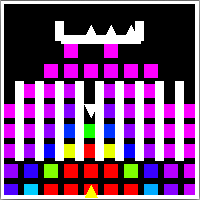
\includegraphics[width=50mm]{resources/hillclimbing2.png}
  \caption{Hill Climbing met afsluiting van pad}
  \label{fig:hillclimbing2}
\end{figure}

\section{Verkenstrategie}

De verkenstrategie is gebaseerd op hetzelfde principe. Hier is er niet \'e\'en bron die een geur uitstuurt, maar iedere onbekende sector stuurt een geur uit. De robot zal hierdoor altijd naar het dichtstbijzijnde en het meest onverkende stuk van het doolhof willen gaan. Daarnaast zorgt dit principe er ook voor dat een robot zal terugkeren op zijn stappen en automatisch terugkeert naar achtergelaten onbekende sectoren. We kunnen stellen dat het algoritme impliciet ``Depth-First-Search"\footnote{\url{http://en.wikipedia.org/wiki/Depth-first_search}} implementeert. Figuur \ref{fig:dfs} toont een robot die een onbekend doolhof aan het verkennen is. De fel groene sectoren zijn onbekende sectoren en hebben een hogere waarde dan de reeds bezochte sectoren.

\begin{figure}[htbp]
  \centering
  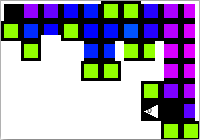
\includegraphics[width=50mm]{resources/dfs.png}
  \caption{Hill Climbing met impliciet ``Depth-First-Search'' zoekgedrag}
  \label{fig:dfs}
\end{figure}

Het toepassen van hetzelfde algoritme voor beide deelproblemen, levert ons in essentie een enkelvoudige implementatie van beide. Door het toekennen van goed gekozen waarden aan onbekende sectoren en aan sectoren waar Pac-Man werd gezien, stelt het algoritme ons in staat om steeds het optimale doel te kiezen. Wanneer er zich geen pad bevindt naar de Pac-Man zal een ``ghost'' onbekende sectoren trachten te verkennen. Wanneer er een pad bestaat naar de Pac-Man zal zijn ``geur'' dit pad nog extra versterken en zal een ``ghost'' automatisch hierdoor aangetrokken worden.

\chapter{Softwaredesign}

In het eerste semester hadden we reeds een redelijk uitgebreid raamwerk opgebouwd om robots samen te stellen uit componenten. Dankzij dit werk kunnen we in het twee semester hier op verder bouwen door de bestaande concepten verder te verfijnen en uit te breiden.

\section{Robot}

Klasse diagram \ref{uml:design-semester1} toont de belangrijkste bouwstenen van ons robot-raamwerk, zoals dit tijdens het eerste semester werd ontworpen: Een Robot-entiteit beschikt over een RobotAPI om met de fysieke robot informatie uit te wisselen. Deze informatie heeft betrekking op de gemeten waarden van de verschillende sensoren als ook het instellen van de motoren. De RobotAPI stelt ons in staat door het vervangen van \'e\'en enkele klasse, om identiek dezelfde Robot-entiteit te gebruiken in een echte fysieke robot, als ook in een gesimuleerde wereld.

\begin{figure}[htbp]
  \centering
  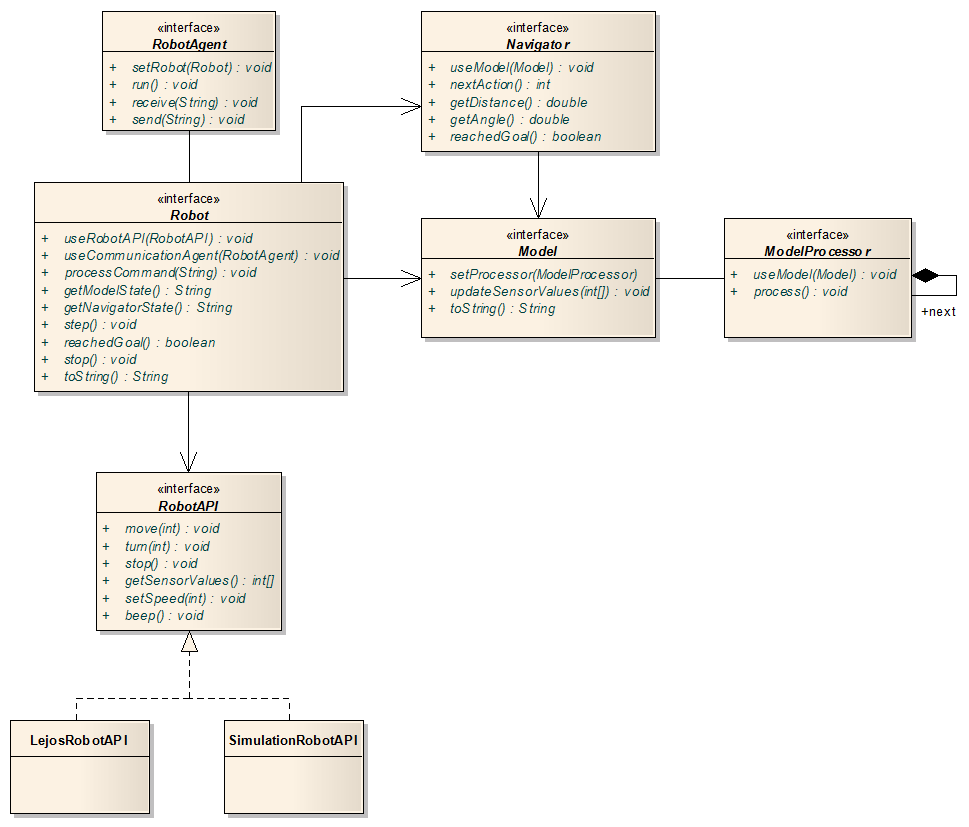
\includegraphics[width=110mm]{resources/design-semester1.png}
  \caption{Design $1^e$ semester}
  \label{uml:design-semester1}
\end{figure}

De Robot beschikt verder over een Model waarin alle informatie uit de wereld wordt samengebracht. Dit model kan verrijkt of bijgewerkt worden door zgn. ModelProcessors. Deze onderzoeken bepaalde delen van het Model en trachten hieruit informatie van een hoger niveau te distilleren. Voorbeelden hiervan zijn processors die op basis van metingen door de sonar-sensor bepalen waar er zich muren bevinden.

Tot slot heeft de Robot ook een Navigator die op basis van de informatie in het Model bepaalt waarheen de Robot dient te rijden. De navigator geeft zeer elementaire instructies aan de Robot, in de vorm van ``beweeg voor- of achterwaarts'' en ``draai zoveel graden''.

Om met de Robot te kunnen communiceren is een RobotAgent voorzien, waarlangs berichten kunnen verzonden en ontvangen worden.

Het is duidelijk dat dit raamwerk een sterk herbruikbare basis biedt om verschillende robots te bouwen. Dit heeft zich al tijdens het eerste semester van nut bewezen, maar komt nog sterker naar voor bij aanvang van het tweede semester. Door het maken van een nieuwe specifieke Navigator en bijhorend Model met Modelprocessors, kunnen we opnieuw een robot samenstellen.

\subsection{Driver}

Ofschoon we een nieuwe Navigator zouden kunnen maken die perfect zou passen, werd snel duidelijk dat er een verfijning van het raamwerk mogelijk was: daar waar tijdens het eerste semester de robot geen resolutie had bij het rijden, is dit in het tweede semester wel het geval. Door het introduceren van het concept van sectoren is er een duidelijk onderscheid tussen het operationele en strategische aspect van het besturen van de robot. Operationeel dient de robot optimaal van sector naar sector te rijden, zodat op strategisch niveau kan geredeneerd worden in termen van deze sectoren.

De functionaliteit om van sector naar sector te rijden zou typisch terecht gekomen zijn in een Navigator-implementatie. Deze wordt in het verfijnde raamwerk ondergebracht in een zgn. ``Driver''. Klasse diagram \ref{uml:design-semster2} toont dat de introductie van de Driver letterlijk een uitbreiding is van het bestaande raamwerk. Voor dit tweede semester is er tevens een eerste implementatie van de Driver gemaakt in de vorm van een ``ManhattanDriver''\footnote{Zo genoemd naar analogie met Manhattan Distance en de Taxicab geometrie: met \url{http://en.wikipedia.org/wiki/Taxicab_geometry}}. 

\begin{figure}[htbp]
  \centering
  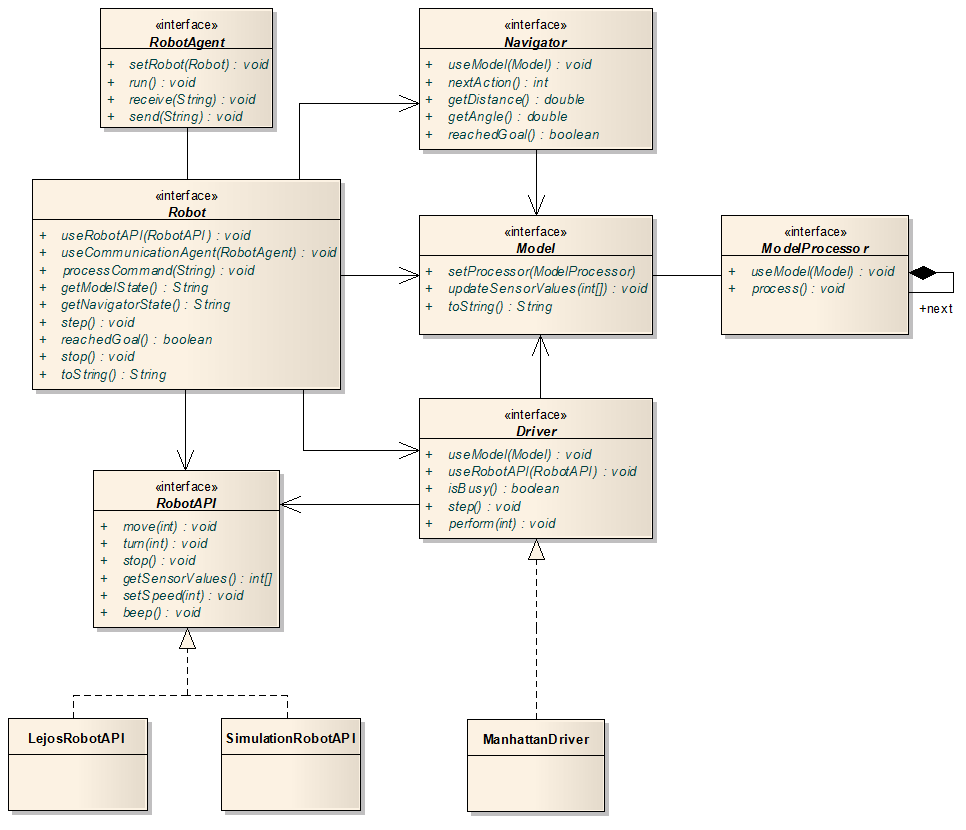
\includegraphics[width=110mm]{resources/design-semester2.png}
  \caption{Design $2^e$ semester}
  \label{uml:design-semster2}
\end{figure}

\subsection{Grids en Sectoren}

De Navigator kan zich nu specifiek toeleggen op het bepalen van de volgende Sector, waarheen de Driver moet rijden. Om deze taak te ondersteunen werden de concepten Grid, Sector en Agent in het leven geroepen. Klasse diagram \ref{uml:grids-sectors} geeft een overzicht van hun samenhang en van de effectieve implementaties die samen de zgn. ``GhostRobot'' opbouwen.

\begin{figure}[htbp]
  \centering
  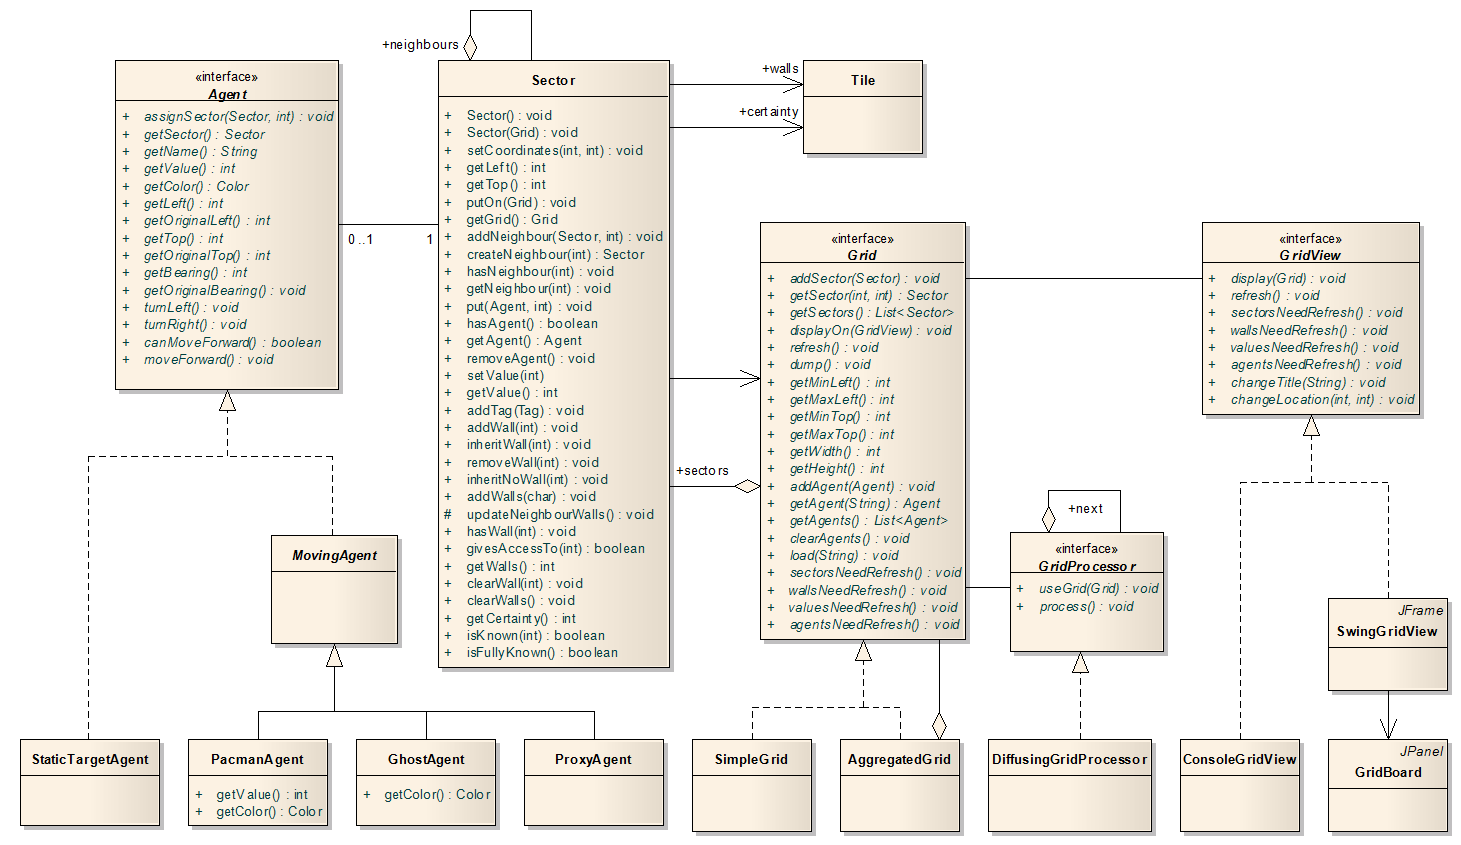
\includegraphics[width=200mm, angle=90]{resources/grids-sectors.png}
  \caption{Design Grids en Sectoren}
  \label{uml:grids-sectors}
\end{figure}

Centraal staat het concept van de Sector in een Grid. Een Sector heeft een co\"ordinaat relatief tov de Grid waarop het zich bevindt, heeft potentieel 4 muren, elk met een bepaalde zekerheid, heeft een waarde en kan bezet worden door een Agent. De waarde van een Sector zal gebruikt worden om de hoogte of de intensiteit van de geur weer te geven. Een Agent kan zich doorheen de Grid bewegen langs de Sectoren. De meeste functionaliteit van een Agent is ge\"implementeerd in een abstracte basis klasse, MovingAgent. Mits kleine configuratie-aanpassingen, implementeren zo de PacmanAgent en de GhostAgent de agents die op de Grid voorkomen. Een ProxyAgent werd gebruikt om in een simulator een echte Agent voor te stellen die de volledige Grid nog niet kent en de StaticTargetAgent werd speciaal voorzien voor de voorbereiding van de eerste demo.

Optioneel kan aan een Grid ook een GridView gegeven worden. Deze voorziet een visualisatie van de Grid en kan op verschillende manieren ingevuld worden. Voor dit project hebben we twee implementaties gemaakt: enerzijds een ConsoleGridView die gedetailleerde informatie over de Sectoren weergeeft en een SwingGridView die een grafische voorstelling geeft van de Grid. Deze laatste wordt gebruikt voor de visualisatie in o.a. de simulator.

Een Grid beschikt ook over een GridProcessor. Net zoals de ModelProcessor kan dit een geschakelde lijst van Processoren zijn die de Grid kunnen ondervragen en bijwerken. Zo hebben we een DiffusionGridProcessor ge\"implementeert die de waarde van de Sectoren zal bijwerken volgens het eerder beschreven algoritme.

De nieuwe robot zal ook informatie van andere robots ontvangen. Deze worden allemaal opgeslagen in een zelfde Grid. Een tweede implementatie van het Grid concept, de zgn. AggregatedGrid, is in staat om een aantal verschillende grids samen in beschouwing te nemen en de ``som'' van deze als een geaggregeerd beeld aan te bieden.

\subsection{GhostRobot}

Klasse diagram \ref{uml:ghostrobot} geeft tot slot de volledige compositie van de nieuwe ``GhostRobot'' weer. De GhostRobot beschikt over een GhostModel, GhostNavigator en GhostDriver.

\begin{figure}[htbp]
  \centering
  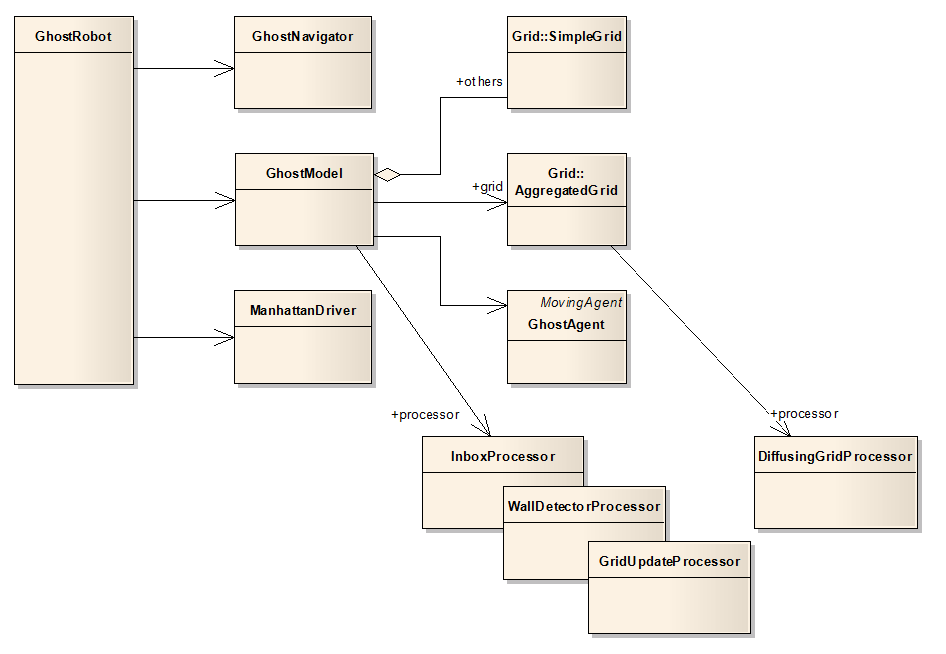
\includegraphics[width=110mm]{resources/ghostrobot.png}
  \caption{Compositie GhostRobot}
  \label{uml:ghostrobot}
\end{figure}

Het GhostModel bevat Grids voor elk van de andere robots alsook een AggregatedGrid voor de eigen Agent. Zolang er geen gemeenschappelijk referentiepunt\footnote{Referentiepunten worden op het parcours voorgesteld door geori\"enteerde barcodes.} is gevonden zijn de verschillende Grids niet met elkaar in verband te brengen. Wanneer er echter een gemeenschappelijk referentiepunt gevonden is, kan de corresponderende Grid van de andere robot toegevoegd worden aan de eigen AggregatedGrid, waardoor de informatie van beide Grids gecombineerd wordt en een ruimer wereldbeeld beschikbaar wordt.

De eigen AggregatedGrid beschikt ook over een DiffusingGridProcessor die het algoritme voor het bepalen van de waarde van een Sector zal toepassen op de AggregatedGrid, waardoor de GhostNavigator een redelijk eenvoudige beslissing kan nemen op basis van de waarden van de vier aangrenzende sectoren.

Het GhostModel is verder voorzien van een aantal ModelProcessoren die de inkomende informatie verwerken tot informatie waarmee de GhostNavigator beslissingen kan nemen. Enerzijds is er een InboxProcessor die de binnenkomende berichten van de andere robots omzet in aanpassingen aan de verschillende Grids in het GhostModel. Anderzijds is er de WallDetectorProcessor die op basis van de gemeten waarden door de sonar-sensor een beeld zal samenstellen van de huidige Sector. Tot slot is er de GridUpdateProcessor die de nieuwe muur-informatie zal verwerken in de eigen Grid en eventueel nieuwe sectoren zal toevoegen.\footnote{Naast deze drie ModelProcessoren zijn er nog andere actief. Het betreft hier bvb. de LineModelProcessor of de WallDetectionModelProcessor. Deze zorgen voor informatie die door de Driver zal gebruikt worden om optimaal naar de volgende sector te rijden. Veel van deze ModelProcessoren maakten reeds deel uit van de robots uit het eerste semester.}

\section{PC}

Aan de zijde van de PC kunnen we opnieuw verder bouwen op onze bestaande ServiceAgent. Naast het logging-kanaal, zal deze nu ook een tweede Bluetooth kanaal volgen, langs het welke de boodschappen van het GhostProtocol kunnen uitgewisseld worden met de Exchange-queue op de RabbitMQ server.

Ook het Dashboard wordt uitgebreid met meer informatie over de werking van het zoek-algortime en de map-verkenning. Hiervoor moet louter bijkomende informatie vanuit het Model en de Navigator doorgestuurd worden, kunnen we Log4J eenvoudig aanpassen in configuratie en voorzien we de databank van bijkomende kolommen om de nieuwe gegevens op te slaan.

Het Dashboard zelf wordt voorzien van de nodige visualisaties voor deze nieuwe informatie. Figuur \ref{fig:dashboard} toont de nieuwe samenstelling.

\begin{figure}[htbp]
  \centering
  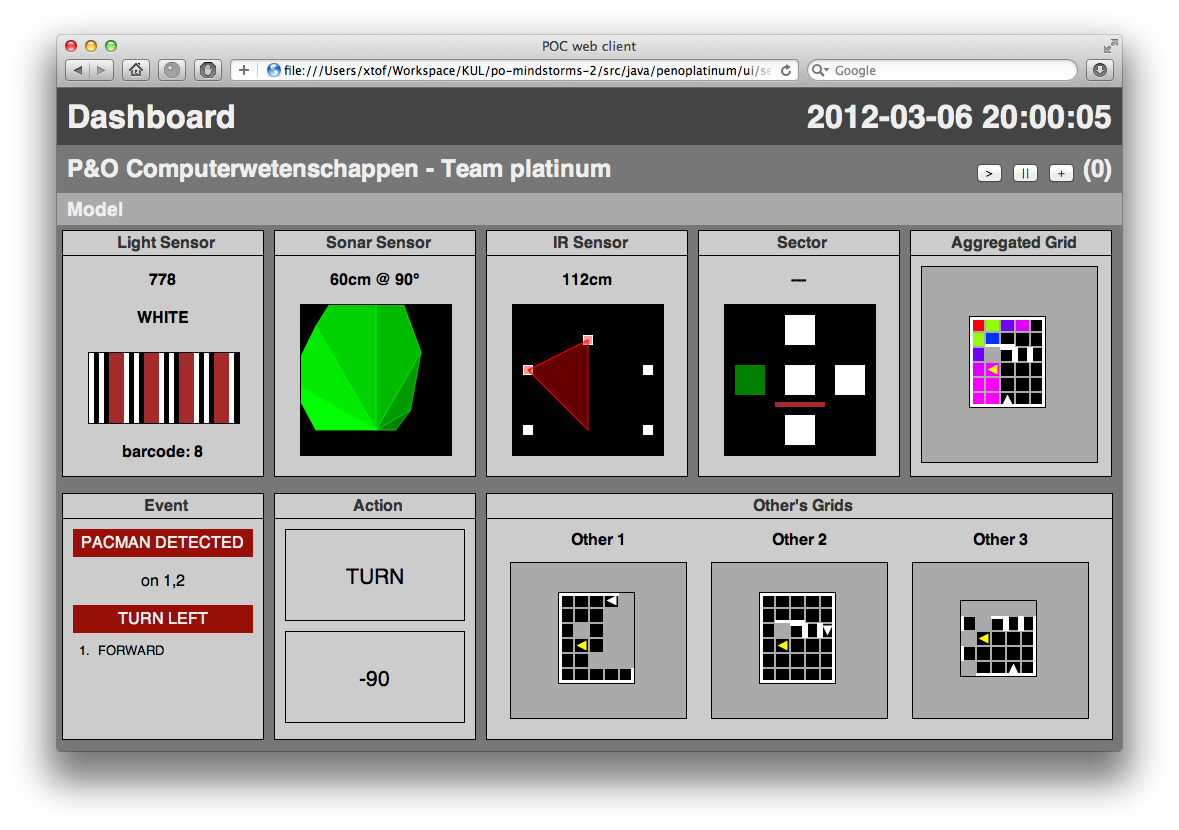
\includegraphics[width=155mm]{resources/dashboard.png}
  \caption{Nieuw Dashboard}
  \label{fig:dashboard}
\end{figure}

\chapter{Simulator}

De simulator is zoals reeds vermeld een verplichte component van het tweede semester en bedoeld als belangrijk hulpmiddel voor de ontwikkeling van de ghosts. Aangezien we tijdens het vorige semester reeds een werkende simulator ontwikkeld hadden, zal deze beschrijving zich vooral focussen op de delen die toegevoegd en/of veranderd werden in functie van de nieuwe opdracht.

Initieel werd er zoveel mogelijk orde geschapen in de bestaande code om zo tot een fase te komen waarbij we de nodige uitbreidingen hebben toegevoegd ter ondersteuning van de nieuwe functionaliteiten. Hierbij moet opgemerkt worden dat de reeds bestaande code werkend is gehouden.

\section{Demo 1}

\subsection{Aanpassingen}

Aangezien de kleinste eenheid van een parcours veranderd is van paneel naar sector, hebben we met behulp van refactoring de simulator aangepast zodat een parcours zowel met panelen als met sectors kan worden voorgesteld. Hierdoor is het mogelijk zowel het project van het eerste semester als het tweede semester uit te voeren. Deze techniek werd verder toegepast op de rest van het herstructureringsproces. 

Naast het aanpassen van de schaal veranderden we ook wijze waarop de verschillende sensoren voorgesteld werden. Op het einde van vorige iteratie waren sensoren eigenlijk functies die elke stap werden opgeroepen om de sensor-waarden in het model up te daten. Deze voorstelling is niet ideaal om uit te breiden. Er werd gekozen voor Sensor interface en voor elke sensor een klasse die deze interface implementeer. Naast een makkelijkere uitbreidbaarheid, heeft dit design ook het voordeel dat men voor elke entiteit zijn eigen sensoren kan aanmaken. En dus een custom mapping kan hebben.

\subsection{Nieuwe Functionaliteit}

Voor het simuleren van meerdere robots, zowel lokaal als op afstand, moest de robot afgescheiden worden van de simulator. Tegelijk werd ook het GUI component van de robot afgescheiden en ge-abstraheerd zodat er meerdere types robots kunnen bestaan. Door deze abstractie is het mogelijk om verschillende simulatoren te laten samenwerken elk met hun eigen robot. Deze simulatoren communiceren met een speciaal protocol op een eigen RabbitMQ kanaal.

Voor het testen van de verschillende algoritmes, specifiek het herori\"entatie algoritme, is er al de mogelijkheid om op sommige plaatsen meet- en stuur-afwijkingen in te voegen in de simulator. De afwijkingen waarop de motor rijdt kan men in de gesimuleerde API van de robot aanpassen, zowel de variantie als een gemiddelde fout kan ingesteld worden, onafhankelijk voor het vooruitrijden en het draaien.

\subsection{Simulator Modi}

De simulator van het eerste semester was een hulpmiddel om met meerdere team-leden in parallel te kunnen werken zonder te moeten strijden om tijd met de echte fysieke robot. In het tweede semester is de simulator een wezenlijk deel geworden van de opdracht en ook de manier waarop de simulator moet kunnen werken is sterk verschillend van onze eigen doelstellingen in het tweede semester.

In het tweede semester moet de simulator op niet minder dan 3 verschillende manieren functioneren:

\begin{itemize}
\item Meerdere (virtuele) robots moeten te gelijkertijd binnen dezelfde simulator aangestuurd kunnen worden.
\item Meerdere instanties van de simulator moeten robots kunnen laten communiceren met elkaar via het Ghost Protocol langs de MQ server.
\item Naast onderlinge communicatie tussen de robots in de simulatoren moeten ook fysieke robots kunnen deelnemen, in een zgn. hybride modus.
\end{itemize}

Figuur \ref{fig:simulator-modi} geeft een overzicht van de verschillende mogelijkheden en hoe deze uitgewerkt zullen worden binnen onze oplossing. De groene pijlen tonen hoe berichten tussen de verschillende robots worden uitgewisseld via het Ghost Protocol en de MQ server. De blauwe pijlen geven aan hoe de informatie over de werking van de robot via de ServiceAgent en het Log4J losging framework opgeslagen worden in de databank, waarna ze ondervraagtaal zijn via de webclient.

\begin{figure}[htbp]
  \centering
  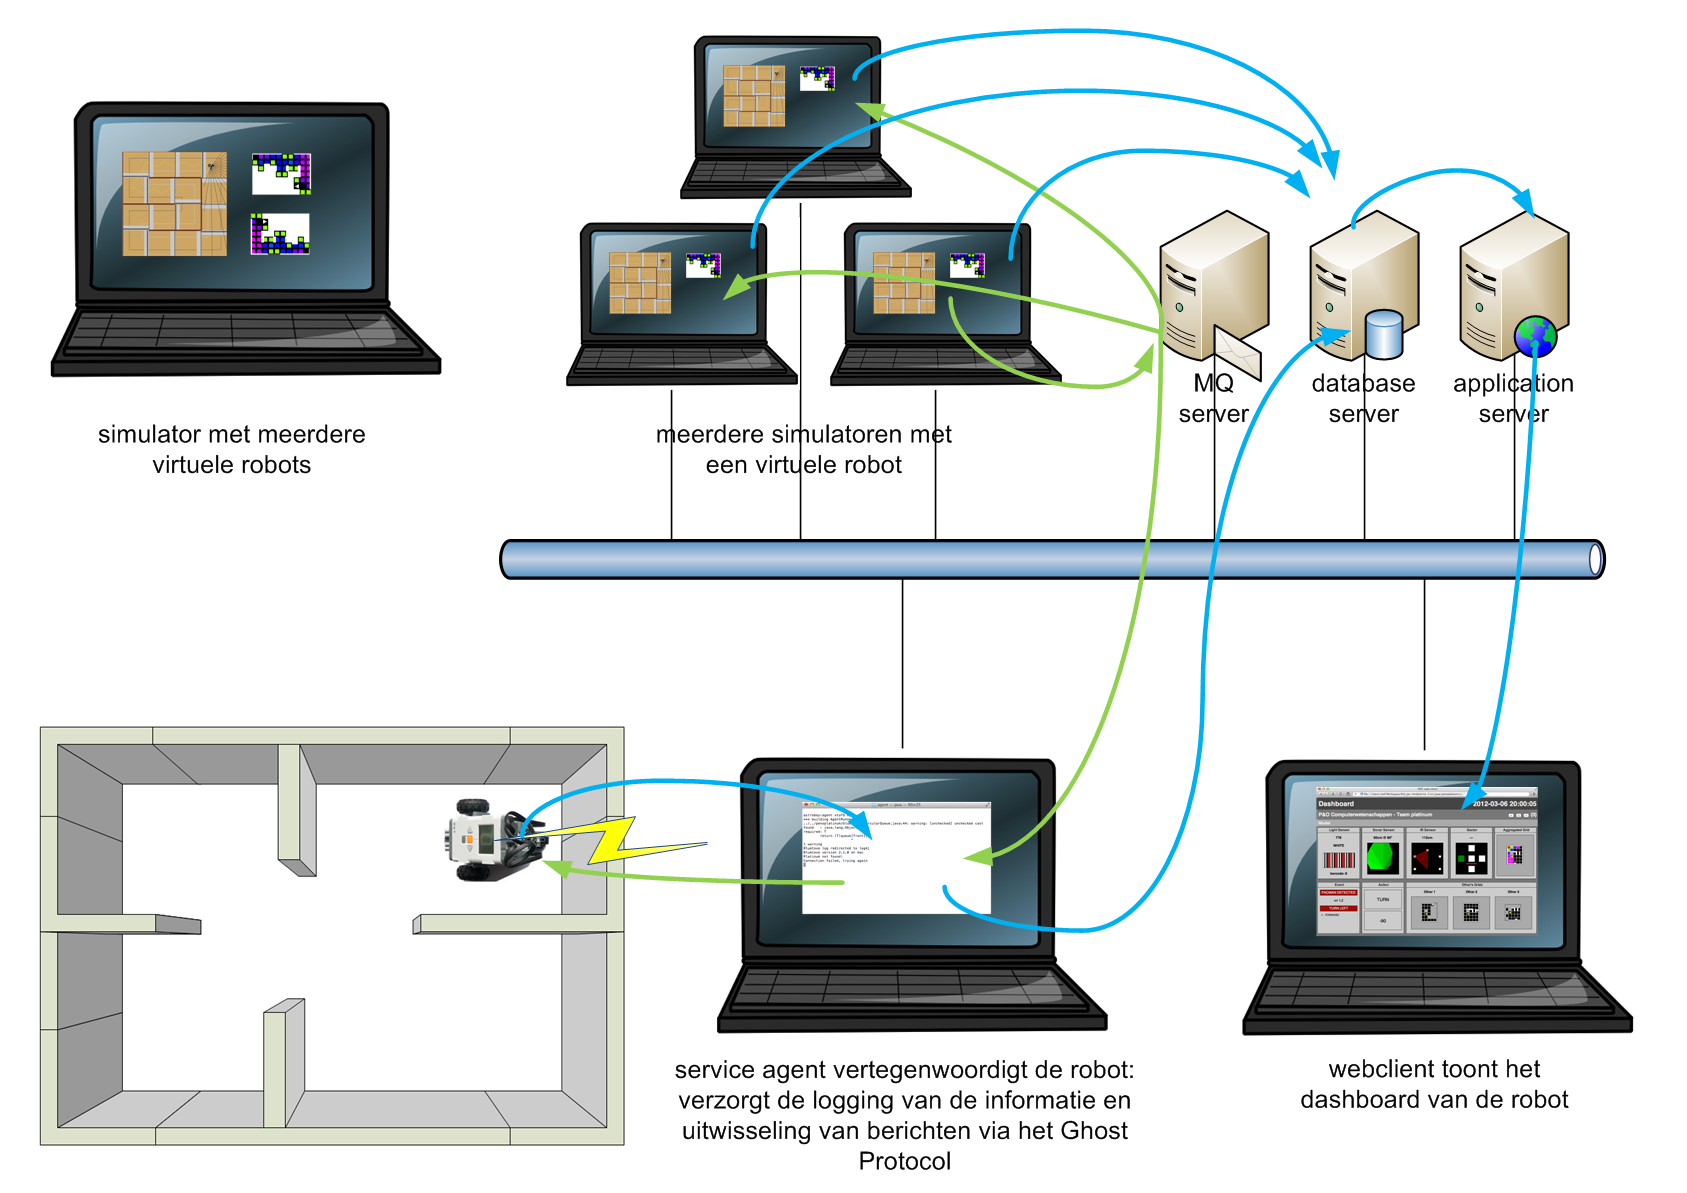
\includegraphics[width=200mm, angle=90]{resources/simulator-modi.png}
  \caption{Werking van de simulator in verschillende opstellingen.}
  \label{fig:simulator-modi}
\end{figure}

\subsection{Mini-Simulator}

Om het onderzoek naar het algoritme onafhankelijk van te laten verlopen van de echte simulator en tevens niet te belasten met details van deze laatste, werd een mini-simulator gemaakt. Deze maakt een abstractie van de wereld en kent alleen een resolutie op niveau van sectoren. Figuur \ref{fig:mini-simulator} toont de mini-simulator in actie met vier gesimuleerde robots, elk vertrokken op een andere positie en met een andere ori\"entatie.

\begin{figure}[htbp]
  \centering
  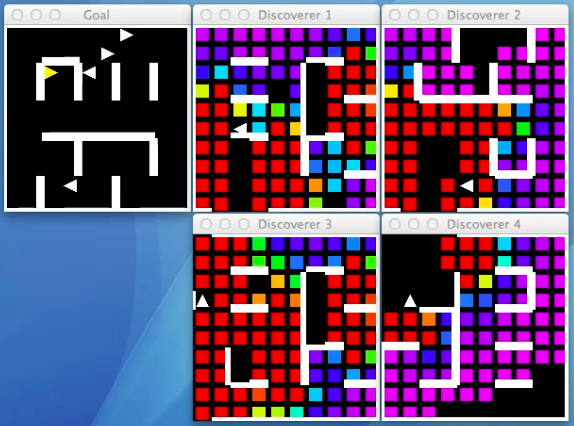
\includegraphics[width=150mm]{resources/mini-simulator.png}
  \caption{Mini-simulator in actie}
  \label{fig:mini-simulator}
\end{figure}

\section{Demo 2}

Dit deel wordt later toegevoegd.

\section{Demo 3}

Dit deel wordt later toegevoegd.

\chapter{Conclusies}

Dit deel wordt later toegevoegd.

\section{Demo 1}

Dit deel wordt later toegevoegd.

\section{Demo 2}

Dit deel wordt later toegevoegd.

\section{Demo 3}

Dit deel wordt later toegevoegd.

\chapter{Procesbeschrijving}

De werkwijze tijdens het eerste semester heeft zijn vruchten afgeworpen. We willen deze aanpak ook in het tweede semester verder zetten. Zo volgen we opnieuw twee paden naar ons doel: enerzijds wordt er verder gewerkt aan de simulator en wordt de robot verder verbetert. Anderzijds starten we ook een traject op dat zich focust op het einddoel.

Omdat de scope van de eerste demo in essentie zo sterkt aanleunt bij het uiteindelijke doel en omdat we met de ontwikkeling van de simulator tijdens het eerste semester een voorsprong hebben tov de over teams willen we trachten om de scope van de finale demo reeds als doelstelling te nemen voor de eerste demo.

Dit gaat hand in hand met de tijd die we ter beschikking hebben tijdens de eerste weken van het semester, wanneer oefenzittingen voor andere vakken nog niet begonnen zijn. We kiezen dus voor een ``blitzkrieg'' waarbij we trachten om de totale scope in een zeer korte tijd te realiseren, waarna we tijdens de resterende weken dit dan verder kunnen verfijnen.

De taken van co\"ordinator (Michiel) en secretaris (Christophe) werden opnieuw verdeeld. Ruben is de nieuwe co\"ordinator. Voor de rol van secretaris werd niet \'e\'en teamlid aangesteld, maar werd besloten om dit een gedeelde taak te maken.

In samenspraak met het didactische team, zal Christophe gedurende twee van de vijf uren die standaard ingepland staan op maandag het team niet vervoegen. Deze uren worden enerzijds onmiddellijk voorafgaandelijk alsook 's avonds na deze vaste uren gepresteerd.

\chapter{Werkverdeling}

\begin{longtable}{l l}
\caption{Focus van elk team lid} \\ [0.5ex]
%This is the header for the first page of the table...
\hline\hline
Teamlid & Focus \\ [0.5ex]
\hline 
\endfirsthead
%This is the header for the remaining page(s) of the table...
\multicolumn{2}{c}{{\tablename} \thetable{} -- Vervolg} \\[0.5ex]
\hline \hline
Teamlid & Focus \\ [0.5ex]
\hline 
\endhead
Michiel 		& 	(Commissie-lid) GhostRobot, Navigator. \\
Florian 		&	Simulator, LightSensor, IR-sensor\\
Ruben 		&	IR-sensor, Simulator\\
Thomas 		&	IR-sensor, Simulator\\
Daniel 		&	Iets? \\
Christophe 	&	Diffusion algoritme, Dashboard \\
\hline
\label{tab:focus}
\end{longtable}

\begin{longtable}{l r r r r r r r}
\caption{Tijdsbesteding per team lid per week} \\
%This is the header for the first page of the table...
\hline\hline
 & Michiel & Florian & Ruben & Thomas & Daniel & Christophe & totaal \\
\hline 
\endfirsthead
totaal & 61 & 38 & 48 & 42 & 22,5 & 63 & 235\\
\hline
week 1 & 12 & 9 & 13 & 12 & 0 & 16,5 & 62,5 \\
week 2 & 16,5 & 14 & 15 & 15 & 10 & 17,5 & 76 \\
week 3 & 32,5 & 21 & 14 & 12,5 & 5 & 29 & 96,5 \\
\hline
gemid./week & 20 & 12 & 16 & 14 & 7,5 & 21 & 13 \\
\label{tab:tijdsregistratie}
\end{longtable}

\chapter{Kritische analyse}

Dit deel wordt later toegevoegd.

\appendix

\chapter{Beoordelingen}

Dit deel wordt later toegevoegd.

\chapter{Grafische User Interface}

Dit deel wordt later toegevoegd.

\chapter{Klasse Diagrammen}

Dit deel wordt later toegevoegd.

\chapter{Planning}
\label{appendix:planning}

Dit deel wordt later toegevoegd.

%Verwijzen naar de docs planning, gedeeld met assistenten.
%Finale demo zal een kopie bevatten.
%\begin{figure}[htbp]
%\centering
%\begin{tikzpicture}
%	\begin{ganttchart}[ 
%	  y unit title=0.6cm,
	  % y unit chart=0.5cm,
	  % vgrid,
	  % bar height=.5,
	  % group right shift=0,
	  % group top shift=.6,
	  % group height=.3]{22}
% \gantttitle{Oktober}{10} 	   	\gantttitle{November}{8} 	    \gantttitle{December}{4} \\
% \gantttitlelist{3,10,17,24,31}{2}	\gantttitlelist{7,14,21,28}{2}  \gantttitlelist{5,12}{2} \\

\end{document}
